\documentclass[11pt,a4paper]{ivoa}
\input tthdefs

\usepackage{xspace}
% Standard terms used throughout the document,
% defined as macro commands to maintain consistency

% Using non-breaking space character.
% https://stackoverflow.com/a/1012891

\newcommand{\xml} {XML}
\newcommand{\json} {JSON}
\newcommand{\yaml} {YAML}

\newcommand{\datamodel} {data~model}
\newcommand{\webservice} {webservice}
\newcommand{\webbrowser} {web browser}

\newcommand{\ivoa} {IVOA}
\newcommand{\uws} {UWS}
\newcommand{\vospace} {VOSpace}

\newcommand{\execplanner} {ExecutionPlanner}
\newcommand{\execworker} {ExecutionWorker}
\newcommand{\executionplanner} {Execution~Planner}

\newcommand{\jupyter} {Jupyter}
\newcommand{\jupyterhub} {JupyterHub}
\newcommand{\binderhub} {BinderHub}

\newcommand{\esap} {ESAP}
\newcommand{\escape} {ESCAPE}
\newcommand{\datalake} {DataLake}
\newcommand{\rucio} {Rucio}

\newcommand{\python} {Python}

\newcommand{\apache} {Apache}
\newcommand{\spark} {Spark}
\newcommand{\pyspark} {PySpark}
\newcommand{\zeppelin} {Zeppelin}

\newcommand{\ocicontainer} {OCI~container}
\newcommand{\docker} {Docker}
\newcommand{\dockercompose} {Docker~compose}
\newcommand{\dockercontainer} {Docker~container}

\newcommand{\codeword}[1] {\texttt{#1}}
\newcommand{\footurl}[1] {\footnote{\url{#1}}}

\newcommand{\dataset} {dataset}
\newcommand{\datascience} {data~science}
\newcommand{\scienceplatform} {science~platform}

\newcommand{\executablething} {\textit{executable~thing}}
\newcommand{\excutabletask} {\textit{task}}
\newcommand{\workerjob} {\textit{job}}

\newcommand{\cpu} {CPU}
\newcommand{\gpu} {GPU}

\usepackage{listings}
\usepackage{xcolor}

\colorlet{punct}{red!60!black}
\definecolor{html-gray}{HTML}{EEEEEE}
\definecolor{light-gray}{gray}{0.95}
\definecolor{delim}{RGB}{20,105,176}
\colorlet{numb}{magenta!60!black}

\lstset{
    basicstyle=\small\ttfamily,
    columns=fullflexible,
    frame=none,
    backgroundcolor=\color{light-gray},
    stepnumber=1,
    %numbers=left,
    numbers=none,
    numberstyle=\small,
    numbersep=8pt,
    %xleftmargin=\parindent,
    xrightmargin=1cm,
    showstringspaces=false,
    keepspaces=true,
    breaklines=true,
    linewidth=14cm,
    frame=none
}

% https://tex.stackexchange.com/questions/83085/how-to-improve-listings-display-of-json-files
% https://tex.stackexchange.com/a/83100
% https://tex.stackexchange.com/questions/10828/indent-a-code-listing-in-latex
% https://tex.stackexchange.com/a/10831
\lstdefinelanguage{json}{
    literate=
     *{0}{{{\color{numb}0}}}{1}
      {1}{{{\color{numb}1}}}{1}
      {2}{{{\color{numb}2}}}{1}
      {3}{{{\color{numb}3}}}{1}
      {4}{{{\color{numb}4}}}{1}
      {5}{{{\color{numb}5}}}{1}
      {6}{{{\color{numb}6}}}{1}
      {7}{{{\color{numb}7}}}{1}
      {8}{{{\color{numb}8}}}{1}
      }

\lstdefinelanguage{yaml}{
    literate=
     *{0}{{{\color{numb}0}}}{1}
      {1}{{{\color{numb}1}}}{1}
      {2}{{{\color{numb}2}}}{1}
      {3}{{{\color{numb}3}}}{1}
      {4}{{{\color{numb}4}}}{1}
      {5}{{{\color{numb}5}}}{1}
      {6}{{{\color{numb}6}}}{1}
      {7}{{{\color{numb}7}}}{1}
      {8}{{{\color{numb}8}}}{1}
      }

\hyphenation{Exe-cut-able-Thing}

\title{IVOA Execution Planner}

% see ivoatexDoc for what group names to use here; use \ivoagroup[IG] for
% interest groups.
\ivoagroup{GWS}

\author[http://www.ivoa.net/twiki/bin/view/IVOA/DaveMorris]
       {Dave Morris}

\editor[http://www.ivoa.net/twiki/bin/view/IVOA/DaveMorris]
       {Dave Morris}

% \previousversion[????URL????]{????Concise Document Label????}
\previousversion{This is the first public release}

\begin{document}
\begin{abstract}

One of the long term goals of the IVOA has been to enable users to
move the code to the data.
This is becoming more and more important as the size and complexity
of the \dataset{}s available in the VO increases.
%\citep{gaia-at-esac}
%\footurl{https://www.skao.int/en/explore/big-data}
%\footurl{https://www.lsst.org/scientists/keynumbers}

The \ivoa{} \executionplanner{} provides a step towards making this possible.

The \ivoa{} \executionplanner{} is designed to address a specific question;
given an \executablething{}, e.g. a \python{} program or a \jupyter{} notebook,
what facilities are available to run it?

To do this, the \ivoa{} \executionplanner{} specification defines
a data model for describing an \executablething{}
and the resources needed to execute it,
and a \webservice{} API for finding platforms
that are able to execute it.

Together these components enable a user to ask a simple question
\textit{"Where (and when) can I execute my program?"}

This in turn enables users to move code between \scienceplatform{}s.
Allowing them to develop their code on one platform and then apply it to a different
\dataset{} by sending it to execute on another platform.

\end{abstract}

\section*{Acknowledgments}

The authors would like to thank all the participants in the IVOA and ESCAPE projects
who have contributed their ideas, critical reviews, and suggestions to this document.

\section*{Conformance-related definitions}

The words ``MUST'', ``SHALL'', ``SHOULD'', ``MAY'', ``RECOMMENDED'', and
``OPTIONAL'' (in upper or lower case) used in this document are to be
interpreted as described in IETF standard RFC2119 \citep{std:RFC2119}.

The \emph{Virtual Observatory (VO)} is a general term for a collection of
federated resources that can be used to conduct astronomical research,
education, and outreach.
The \href{https://www.ivoa.net}{International Virtual Observatory Alliance (IVOA)}
is a global collaboration of separately funded projects to develop standards and
infrastructure that enable VO applications.

\section{Introduction}
\label{sec:introduction}

The \ivoa{} \executionplanner{} specification defines two \webservice{} interfaces,
the \execplanner{} and the \execworker{}, and a common \datamodel{} for describing
executable tasks.

Together these provide a common interface for service discovery, resource allocation
and execution scheduling across a heterogeneous federation of different types of
execution platform.

\begin{itemize}
    \item \execplanner{} \webservice{} – a discovery service to find execution platforms, allocate resources and schedule execution.
    \item \execworker{} \webservice{} – an asynchronous service for executing tasks (based on the \ivoa{} \uws{} pattern).
    \item \execplanner{} \datamodel{} – a common data model for describing \executablething{}s and their resource requirements.
\end{itemize}

\subsection{Role within the VO Architecture}
\label{subsec:ivoarole}

% As of ivoatex 1.2, the architecture diagram is generated by ivoatex in
% SVG; copy ivoatex/archdiag-full.xml to role_diagram.xml and throw out
% all lines not relevant to your standard.
% Notes don't generally need this.  If you don't copy role_diagram.xml,
% you must remove role_diagram.pdf from SOURCES in the Makefile.
\begin{figure}
\centering
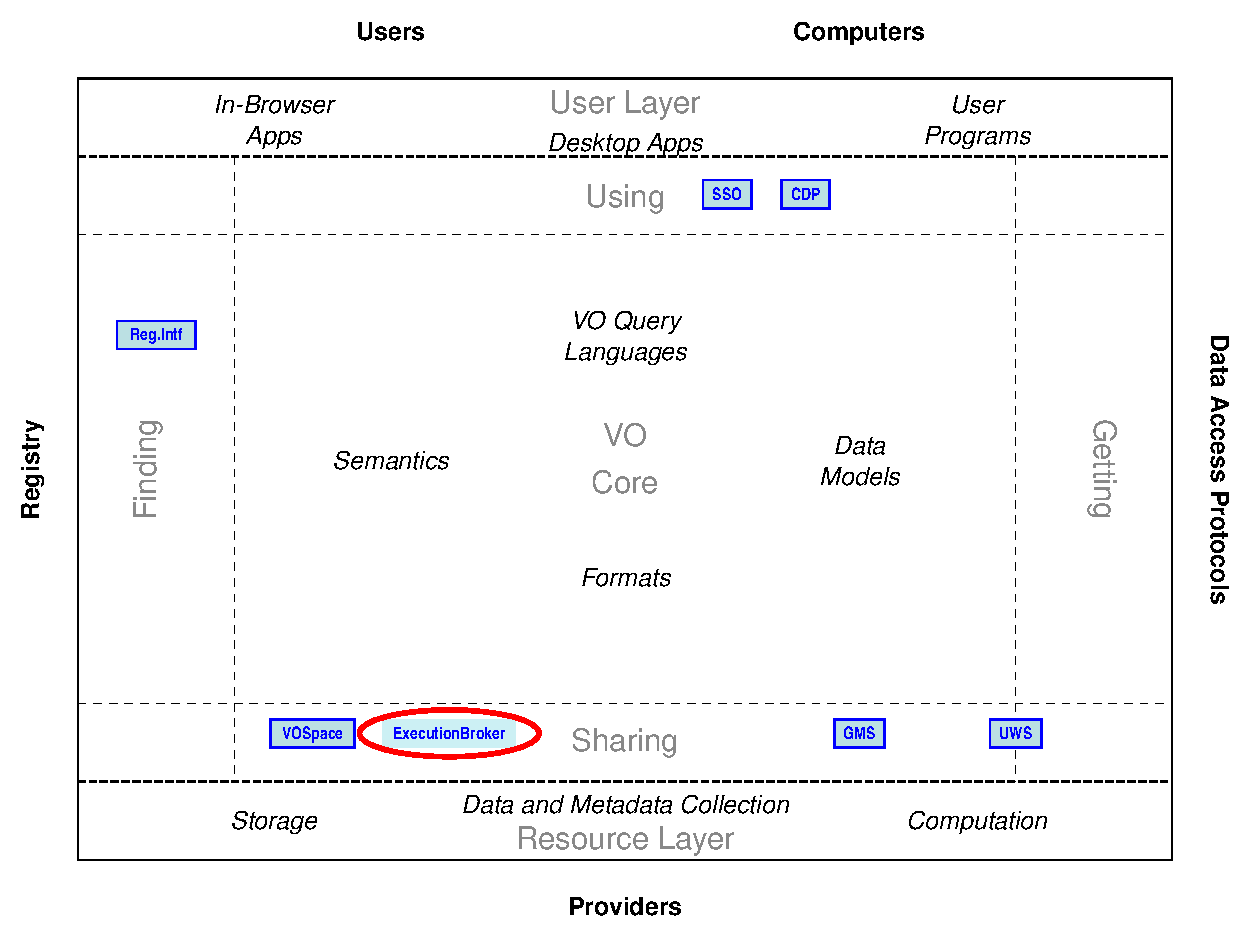
\includegraphics[width=0.9\textwidth]{role_diagram.pdf}
\caption{Architecture diagram showing the \ivoa{} \executionplanner{}'s role in the \ivoa}
\label{fig:archdiag}
\end{figure}

The IVOA Architecture \citep{2010ivoa.rept.1123A} provides a high-level view of how IVOA
standards work together to connect users and applications with providers of data
and services.
Fig.~\ref{fig:archdiag} shows the role the \ivoa{} \executionplanner{} plays within the this architecture.

In response to the increasing size and complexity of the next generation of science \dataset{}s
a number of \ivoa{} members are developing intergrated \scienceplatform{}s which bring
together the \dataset{}s co-located with the compute resources needed to analyse them.
\footurl{https://data.lsst.cloud/}
\footurl{https://rsp.lsst.io/index.html}

The \scienceplatform{}s make extensive use of the \ivoa{} data models and
vocabularies to describe their \dataset{}s, and use the \ivoa{} data access
services to find and access data from other data providers.
In addition, some of the \scienceplatform{}s use \ivoa{} \vospace{} services to manage
data transfers to and from local storage co-located with the compute resources.

However, to date the \ivoa{} does not provide any APIs or \webservice{} interfaces that
enable \scienceplatform{}s to exchange the software used to analyse the data.
The \ivoa{} \executionplanner{} provides a step towards making this possible.

This places the \ivoa{} \executionplanner{} in the same region of the \ivoa architecture
as the \ivoa{} \vospace{} specification \citep{2009ivoa.specQ1007G},
providing an infrastructure level service that enables service discovery,
resource allocation and execution scheduling across a heterogeneous federation
of execution platforms.

The \ivoa{} \executionplanner{} specification refers to the
\ivoa Single-Sign-On standard \citep{2017ivoa.spec.0524T}
for authentication (see section xx )%\ref{subsec:authentication}
and the
\ivoa Credential Delegation Protocol \citep{2010ivoa.spec.0218P}
for delegating credentials to other services.

The \ivoa{} \executionplanner{} specification also describes how to register
an \execplanner{} service in the
\ivoa{} Registry \citep{2009ivoa.spec.1104B}
making it findable within the wider context of the VO.

\subsection{Executable things}
\label{subsec:executablething}

To understand the problem that \ivoa{} \executionplanner{} is trying to solve
it is useful to describe what an \executablething{} means in this context.

If we start by thinking of a science domain function that we want to perform.
For example, the mathematical concept of the square root of a number.
We can calculate the square root of a positive number using the Newton–Raphson algorithm
\footurl{https://en.wikipedia.org/wiki/Newton\%27s_method}
which produces successively closer approximations to the result.

We can write a \python{} program to use this algorithm to calculate the square root of a number.
This is the first identifiable \executablething{} in our example.
To be able to use this \executablething{} you would need a computing resource with the appropriate
hardware and software environment. In this case, a computing resource with the \python{} interpreter
installed along with any 3rd \python{} modules equired by the program.
This environment is often referred to as the \textit{\python{} runtime}.

In the context of \scienceplatform{}s and \datascience{}, a common pattern is to provide this environment
using an \ocicontainer{}\footurl{https://opencontainers.org/},
or \dockercontainer\footurl{https://docs.docker.com/get-started/what-is-a-container/},
to package the \python{} program and the \python{} runtime together as a single binary object.
This package, or container, is itself an \executablething{}. One which requires a different execution
environment than the original \python{} program.
The key concept behind containerization is to package programs together with the software environment
they need as single binary object that interfaces with a standard execution environment,
referred to as the \textit{container runtime} or \textit{container engine}.
To be able to use this \executablething{} you would need a computing resource with the appropriate
hardware and software environment. In this case, a computing resource with the OCI container runtime installed.

We could also create a \jupyter{} notebook that demonstrates how to use our \python{} program.
This is the third \executablething{} in our example.
One which provides an interactive environment for the user to experiment with.
As before, to be able to use this \executablething{} we would need a computing resource with
the appropriate hardware and software environment.
In this case, a computer with the \jupyter{} notebook platform installed along with all the 3rd \python{} modules
needed by our \python{} program.
In the context of \scienceplatform{}s and \datascience{}, a common pattern is to provide this environment as a \webservice{}
that allows the user to connect to the \jupyter{} notebook via a \webbrowser.

From one algorithm that implements a science domain function, we have created three different \executablething{}s.
A \python{} program, an \ocicontainer{} packaging the \python{} program and its dependencies, and an interactive \jupyter{} notebook
that demonstrates how to use the \python{} progran.

Each of these \executablething{}s requires a different computing environment to execute.
A basic \python{} runtime, the \ocicontainer{} runtime, and a \jupyter{} notebook service.

We may also want to consider the data that we are applying the algorithm to.
If we are learning how to use algorithm, then a basic computing resource will be sufficient
to experiment with.
However, if we have a \dataset{} of ten million numbers that we want to process, then we may
need to consider adding extra storage to handle the input data and the results.
For a large \dataset{} it may also be worth using a \gpu{} to accelerate the calculation steps
for such a large \dataset{}.

The \ivoa{} \executionplanner{} \datamodel{} provides a way to describe what each of these \executablething{}s
is and what resources are needed to execute them.
This can include things like number of \cpu cores and amount of memory it needs,
whether it needs a \gpu{}, the location of the input data, the storage space needed to perform
the calculation and the storage space needed to save the results.
For details on the \ivoa{} \executionplanner{} \datamodel{} see appendix xx.

In the context of this document, we will use the term \excutabletask{} to refer to the metadata
describing an \executablething{} and the resources needed to execute it.
This \excutabletask{} description can be passed to an \ivoa{} \executionplanner{} service to
discover if the service is able to provide the resources required to execute this particular
\executablething{}.

\section{Client-server conversation}
\label{sec:conversation}

The core idea behind the \ivoa{} \executionplanner{} is based on a conversation between the client
and one or more \execplanner{} services to discover where, how, and when, an \excutabletask{} can be
executed.

The conversation starts with the client sending a description of the \excutabletask{} to each of the
\execplanner{} services, which respond with a top level \codeword{YES|NO} answer, and if
the answer is \codeword{YES}, a list of offers describing where how, and when, the \excutabletask{}
can be executed on their platform.

Given a list of offers from the \execplanner{} services, the client can choose which of the offers it
wants to use and sends a reply to that \execplanner{} service accepting the offer.
In response the \execplanner{} will cancel any other offers it made, mark the resources descibed in the accepted
offer as reserved, initiate a \workerjob{} in an \execworker{} service to execute the \excutabletask{}
and reply with details of how to access the \workerjob{}.

The client can then uses the connection details in the response to contact the \execworker{} service that
is executing the \excutabletask{} to track the status of the job.
For further details of the \webservice{} request and response messages see section xxx.

Note that the client does not need to cancel the offers made by the other \execplanner{} services.
Offers are only valid for a limited period of time, and expire naturally when they reach the end
of their lifetime.

\subsection{'Can I ..?' questions}
\label{subsec:questions}

The content of the \excutabletask{} description is best explained by considering a series of
questions that can be used to discover where how, and when, to execute a \excutabletask{}.

\subsubsection{Level 1 - the \excutabletask{}}
\label{subsubsec:thetask}

At the simplest level we just want to check whether a platform is able to execute a particular
type of \excutabletask{}.
For example, \textit{"Is this platform able to run a \jupyter{} notebook?"}

In order to do this, the request needs to specify the task type, e.g. \jupyter{} notebook,
along with details about it, e.g. where to fetch the notebook from.

The metadata for this part of the \excutabletask{} description is different for each type of task.
Rather than try to model every possible type of task, the metadata for each task type is described by
an extension to the core \datamodel{}.

To support this pattern the core \executionplanner{} \datamodel{} has two fields, \codeword{type},
a URI identifying the task type, and \codeword{spec}, a place holder for details about the task.

\begin{lstlisting}[language=yaml]
task:
  # A URI identifying the basic type of task.
  # e.g.
  # https://www.purl.org/ivoa.net/ep/task-type/oci-container
  # https://www.purl.org/ivoa.net/ep/task-type/jupyter-notebook
  type: "https://www.purl.org/ivoa.net/ep/task-type/example"

  # The task details, specific to the task-type.
  spec: {}
\end{lstlisting}

The \datamodel{} extension for a task type defines the metadata needed to describe that particular type of task.
For example, the \datamodel{} extension for a \jupyter{} notebook needs to describe where to fetch the source code for the notebook from.
\begin{lstlisting}[language=yaml]
task:
  # A URI identifying the basic type of task.
  type: "https://www.purl.org/ivoa.net/ep/task-type/jupyter-notebook"

  # The task details, specific to the task-type.
  spec:
    notebook: "https://.../example.jpnb"
\end{lstlisting}

It may also include a reference to a \codeword{requirements.txt} file that describes any additional \python{}
libraries needed by the notebook.
\begin{lstlisting}[language=yaml]
task:
  # A URI identifying the basic type of task.
  type: "https://www.purl.org/ivoa.net/ep/task-type/jupyter-notebook"

  # The task details, specific to the task-type.
  spec:
    notebook: "https://.../example.jpnb"
    requirements: "https://.../requirements.txt"
\end{lstlisting}

The \datamodel{} extension for an \ocicontainer{} task needs to describe what operating system and system architecture
the container is is built for, and where to fetch the binary image from.

\begin{lstlisting}[language=yaml]
task:
  # A URI identifying the basic type of task.
  type: "https://www.purl.org/ivoa.net/ep/task-type/oci-container"

  # The task details, specific to the task-type.
  spec:
    os:    "linux"
    arch:  "amd64"
    repo:  "ghcr.io"
    image: "ivoa/oligia-webtop"
    version: "ubuntu-2022.01.13"
\end{lstlisting}

The \executionplanner{} specification defines an initial set of common task types, e.g. \ocicontainer{}, \jupyter{} notebook,
and \zeppelin{} notebook.
The extension pattern is designed to make it easy for 3rd parties to develop new types of tasks appropriate for their science domain.

Using the \codeword{type} URI to identify the task type means that service implementations do not need to understand
all of the different possible task types that a client could request.
A service that doesn’t recognize a particular task type can simply reply \codeword{NO}.

\begin{lstlisting}[]
Request  - Can this platform execute <unkown-task-type> ?
Response - NO
\end{lstlisting}

For a full listing of the task types included see appendix xxx.

TODO some text about using URIs ...



\appendix
\section{Changes from Previous Versions}

No previous versions yet.
% these would be subsections "Changes from v. WD-..."
% Use itemize environments.


% NOTE: IVOA recommendations must be cited from docrepo rather than ivoabib
% (REC entries there are for legacy documents only)
\bibliography{ivoatex/ivoabib,ivoatex/docrepo}


\end{document}
